\documentclass[
  bibliography=totoc,     % Literatur im Inhaltsverzeichnis
  captions=tableheading,  % Tabellenüberschriften
  titlepage=firstiscover, % Titelseite ist Deckblatt
  parskip=half, % !!! halbzeiliger vertikaler Abstand (siehe Latex-Skript S.125)
]{scrartcl}

% !!! Python in Latex
\usepackage{pythontex}

% !!! zum Drehen von Seiten
\usepackage{adjustbox}

% Paket float verbessern
\usepackage{scrhack}

% Warnung, falls nochmal kompiliert werden muss
\usepackage[aux]{rerunfilecheck}

% unverzichtbare Mathe-Befehle
\usepackage{amsmath}
% viele Mathe-Symbole
\usepackage{amssymb}
% Erweiterungen für amsmath
\usepackage{mathtools}

% Fonteinstellungen
\usepackage{fontspec}
% Latin Modern Fonts werden automatisch geladen
% Alternativ zum Beispiel:
%\setromanfont{Libertinus Serif}
%\setsansfont{Libertinus Sans}
%\setmonofont{Libertinus Mono}

% Wenn man andere Schriftarten gesetzt hat,
% sollte man das Seiten-Layout neu berechnen lassen
\recalctypearea{}

% deutsche Spracheinstellungen
\usepackage[ngerman]{babel}

% !!! babel mit anderen Sprachen laden für \enquote (siehe latex-Skript S.33)
\usepackage[autostyle]{csquotes}

% !!! zum durchstreichen durch \cancel{}
\usepackage[makeroom]{cancel}

% !!! zum Ersetzen von \symup{} durch z.B. \dif{} (siehe latex-Skript)
\usepackage{expl3}
\usepackage{xparse}
\ExplSyntaxOn
\NewDocumentCommand \dif {m} {
  \mathinner{\symup{d} #1}
}
\ExplSyntaxOff

% !!! Nummerierung von Gleichungen nach Sections: Bei langen Dokumenten empfohlen
% \numberwithin{equation}{section}


\usepackage[
  math-style=ISO,    % ┐
  bold-style=ISO,    % │
  sans-style=italic, % │ ISO-Standard folgen
  nabla=upright,     % │
  partial=upright,   % ┘
  warnings-off={           % ┐
    mathtools-colon,       % │ unnötige Warnungen ausschalten
    mathtools-overbracket, % │
  },                       % ┘
]{unicode-math}

% traditionelle Fonts für Mathematik
\setmathfont{Latin Modern Math}
% Alternativ zum Beispiel:
%\setmathfont{Libertinus Math}

\setmathfont{XITS Math}[range={scr, bfscr}]
\setmathfont{XITS Math}[range={cal, bfcal}, StylisticSet=1]

% Zahlen und Einheiten
\usepackage[
  locale=DE,                   % deutsche Einstellungen
  separate-uncertainty=true,   % immer Unsicherheit mit \pm
  per-mode=symbol-or-fraction, % / in inline math, fraction in display math
]{siunitx}

% chemische Formeln
\usepackage[
  version=4,
  math-greek=default, % ┐ mit unicode-math zusammenarbeiten
  text-greek=default, % ┘
]{mhchem}

% richtige Anführungszeichen
\usepackage[autostyle]{csquotes}

% schöne Brüche im Text
\usepackage{xfrac}

% Standardplatzierung für Floats einstellen
\usepackage{float}
\floatplacement{figure}{htbp}
\floatplacement{table}{htbp}

% Floats innerhalb einer Section halten
\usepackage[
  section, % Floats innerhalb der Section halten
  below,   % unterhalb der Section aber auf der selben Seite ist ok
]{placeins}

% Seite drehen für breite Tabellen: landscape Umgebung
\usepackage{pdflscape}

% Captions schöner machen.
\usepackage[
  labelfont=bf,        % Tabelle x: Abbildung y: ist jetzt fett
  font=small,          % Schrift etwas kleiner als Dokument
  width=0.9\textwidth, % maximale Breite einer Caption schmaler
]{caption}

% subfigure, subtable, subref
\usepackage{subcaption}

% Grafiken können eingebunden werden
\usepackage{graphicx}

% !!! Textumflossene Grafiken
\usepackage{wrapfig}

% !!! Kreisnummern
\usepackage{tikz} 

% !!! größeres Seitenlayout für mehr Platz
\usepackage[a4paper, left=30mm, top=30mm, right=30mm, bottom=40mm]{geometry} 

% !!! Aufgaben nummerieren
\usepackage{tasks}

% !!! Für das Einfügen von pdfs wie Messdaten etc.
\usepackage{pdfpages}

% schöne Tabellen
\usepackage{booktabs}

% Verbesserungen am Schriftbild
\usepackage{microtype}

\usepackage{rotating}
% Literaturverzeichnis
\usepackage[
  backend=biber,
]{biblatex}
% Quellendatenbank
\addbibresource{lit.bib}
\addbibresource{programme.bib}

% Hyperlinks im Dokument
\usepackage[
  english,
  unicode,        % Unicode in PDF-Attributen erlauben
  pdfusetitle,    % Titel, Autoren und Datum als PDF-Attribute
  pdfcreator={},  % ┐ PDF-Attribute säubern
  pdfproducer={}, % ┘
]{hyperref}
% erweiterte Bookmarks im PDF
\usepackage{bookmark}

% Trennung von Wörtern mit Strichen
\usepackage[shortcuts]{extdash}

\author{%
  Celina Kortmann\\%
  \href{mailto:celina.kortmann@tu-dortmund.de}{celina.kortmann@tu-dortmund.de}%
  \and%
  Jan Lucca Viola\\%
  \href{mailto:janlucca.viola@tu-dortmund.de}{janlucca.viola@tu-dortmund.de}%
}
\publishers{TU Dortmund – Faculty of Physics}
\setlength\parindent{0pt}

\subject{V47}
\title{Molar heat of Cu}
\date{
  Experiment date: May 6th, 2024
  \hspace{3em}
  Submission: May 6th, 2024
}

\begin{document}

\maketitle
\thispagestyle{empty}
\tableofcontents
\newpage
\setcounter{page}{1}
\section{Introduction}
\label{sec:Ziel}
\section{Theory}
\label{sec:theory}

The molar heat describes the quantity of heat, that is needed to warm one Mol by one Kelvin. This is characterized by the formula 
\begin{equation*}
    C = \frac{\Delta Q}{\Delta T} \,\, . 
\end{equation*}
The molar heat can be reduced to the pressure or to the volume. In this experiment we measure the molar heat with a constant pressure $C_{\symup{p}}$. 
For a constant volume a very high pressure would be needed. We can transform $C_{\symup{p}}$ to $C_{\symup{V}}$ by using 
\begin{equation}
    C_{\symup{V}} = C_{\symup{p}} - 9{\alpha}^2\kappa V_{\symup{0}}T \,\, .
    \label{eqn:CV}
\end{equation}
Here $\alpha$ describes the expansion coefficient and $\kappa$ the compressibilities.
The Debye temperature we mentioned before is material specific and depends on the phonon frequency. If the temperature is below this Debye temperature,
we have to consider quantum effects just as freezing of degrees of freedom. Above the Debye temperature all natural vibration states are occupied. 

\subsection{Classical theory of the molar heat}
\label{sec:classic}
In a solid, the energy is equally distributed on its degrees of freedom. A solid has six degrees of freedom, three for translation and three for rotation.
Each atom has an energy of $\frac{1}{2}\symup{k_B}T$ per degree of freedom. So the overall the energy is $E=3\symup{k_B}T$, where $\symup{k_B}$ 
is the Boltzmann constant. For one Mol we get 
\begin{equation*}
    E = 3\symup{k_B}\symup{N_A}T = \symup{R}T \,\, ,
\end{equation*}
where $\symup{N_A}$ is the Avogadro constant and $\symup{R}$ is the general gas constant. If we describe the specific heat capacity at a constant volume, 
we get the Dulong-Petit law
\begin{equation*}
    C_V = \left.\frac{\symup{\partial}U}{\symup{\partial}T}\right|_V=3 \symup{R} \,\, .
\end{equation*}
The Dulong-Petit law does not depend on material or temperature. At low temperatures measurements show no agreement. A classical description 
only approximates high temperatures ($T>> \symup{\theta_D}$).

\subsection{The Einstein model}
\label{sec:einstein}
The Einstein model takes quantum effects into account. It describes the solid as an oscillator. All oscillations are assumed to have the
uniform frequency $\omega_E$. Einstein considers the quantization of energy, which he assumes can only change in $\hbar \omega_E$. 
The Boltzmann distribution 
\begin{equation*}
    W(n)= \symup{exp}\left(-\frac{n\hbar \omega_E}{\symup{k_B}T}\right)
\end{equation*}
describes the probability that the oscillator has the energy $n\hbar\omega_E$ (n $\in$ N) at a given temperature. 
The mean energy is calculated by a summation and a normalization of all possible energies
\begin{equation*}
    \langle E \rangle = \frac{\hbar \omega_E}{\symup{exp} \left(\frac{\hbar \omega E}{\symup{k_B}T}\right)-1} \,\, .
\end{equation*}
With the Einstein temperature 
\begin{equation*}
    \symup{\theta_E} = \frac{\hbar \omega_E}{\symup{k_B}}
\end{equation*}
the molar heat at a constant volume can be depicted by 
\begin{equation*}
    C_V = 3\symup{N_A k_B}\left(\frac{\symup{\theta_E}}{T}\right)^2 \frac{\symup{e}^{\symup{\theta_E}/T}}{\left(\symup{e}^{\symup{\theta_E}/T}-1\right)^2} \,\, .
\end{equation*}
If we approximate the molar heat for very low and very high temperatures we get 
\begin{equation*}
    C_V = 
    \begin{cases}
        3 \symup{R}\left(\frac{\symup{\theta_E}}{T}\right)^2 \frac{\symup{e}^{\symup{\theta_E}/T}}{\left(\symup{e}^{\symup{\theta_E}/T}-1\right)^2} , & T << \symup{\theta_E} \\
        3 \symup{R} , T >> \symup{\theta_E}
    \end{cases}
    \, \, .
\end{equation*}
Again, for high temperatures we get the Dulong-Petit law, which approximates the experimental capacity good. For low temperatures we expect 
a $T^3$-dependence at the real measured values, that is not described by the Einstein model.

\subsection{The Debye model}
\label{sec:debye}
The Debye model introduces a spectral distribution $Z(\omega)$. With the Debye wave vector $q_D$ we get a linear dispersion
$\omega_i = v_i q_D$ for three branches $i$ with phase velocity $v_i$. For a crystal with a finite number of atoms $\symup{N_A}$ the 
number of oscillation frequencies is also finite. We get one frequency for each atom and each spatial direction, so that we have a total 
of $3\symup{N_A}$ oscillation frequencies. The surfaces of the same frequency are spherical surfaces with a volume of $\left(\frac{2\pi}{L}\right)^2$, 
so that we get the Debye wave vector 
\begin{equation*}
    q_D = \left(6\pi^2\frac{\symup{N_A}}{V}\right)^{1/3} \,\,. 
\end{equation*}
The Debye frequency is given by 
\begin{equation*}
    \omega_D = q_D v_i = v_i \left(6\pi^2 \frac{\symup{N_A}}{V}\right)^{1/3} \,\, .
\end{equation*}
The molar heat capacity at a constant volume can be calculated as 
\begin{equation*}
    C_V = 9\symup{N_A k_B}\left(\frac{T}{\symup{\theta_D}}\right)^3 \int_{0}^{\symup{\theta_D}/T}\frac{x^4\symup{e}^x}{\left(\symup{e}^x-1\right)^2}\, \symup{d}x \,\, .
\end{equation*}
Here the Debye temperature is defined as
\begin{equation}
    \symup{\theta_D} = \frac{\hbar \omega_D}{\symup{k_B}} = \frac{\hbar v_{eff}}{\symup{k_B}}\left(6\pi^2\frac{\symup{N_A}}{V}\right)^{1/3}
    \label{eqn:theoDebye}
\end{equation}
with the effective spead of sound $v_{eff}$ \
\begin{equation*}
    v_{eff}^3 = 3 \frac{v_l^3 v_t^3}{v_t^3 + 2v_l^3}
\end{equation*}
The approximation for very low and very high temperatures is given by 
\begin{equation*}
    C_V = 
    \begin{cases}
        \frac{12\pi^4}{5}\symup{R}\left(\frac{T}{\symup{\theta_D}}\right)^3 , & T << \symup{\theta_D} \\
        3\symup{R} , & T>> \symup{\theta_D}
    \end{cases}
    \,\, .
\end{equation*}
The dependence for high temperatures equals the Dulong-Petit law again. For low temperatures the $T^3$-dependence is correctly pictured by 
the Debye model.

\subsection{Calculation of $C_p$}
The molar heat at a constant pressure can be calculated by 
\begin{equation}
    C_p = \frac{M}{m} \cdot \frac{E}{\Delta T} \,\, , 
    \label{eqn:Cp}
\end{equation}
where $M$ is the molecular weight and $m$ is the weight of the sample. 
The supplied energy $E$ is determined by 
\begin{equation*}
    E = U \cdot I \cdot \Delta t
\end{equation*}
\section{Implementation}
\label{sec:Aufbau}

\subsection{Setup}
For this experiment, which is used to determine the molar heat capacity of copper, the apparatus shown in \autoref{fig:Aufbau} is needed.
\begin{figure}
    \centering
        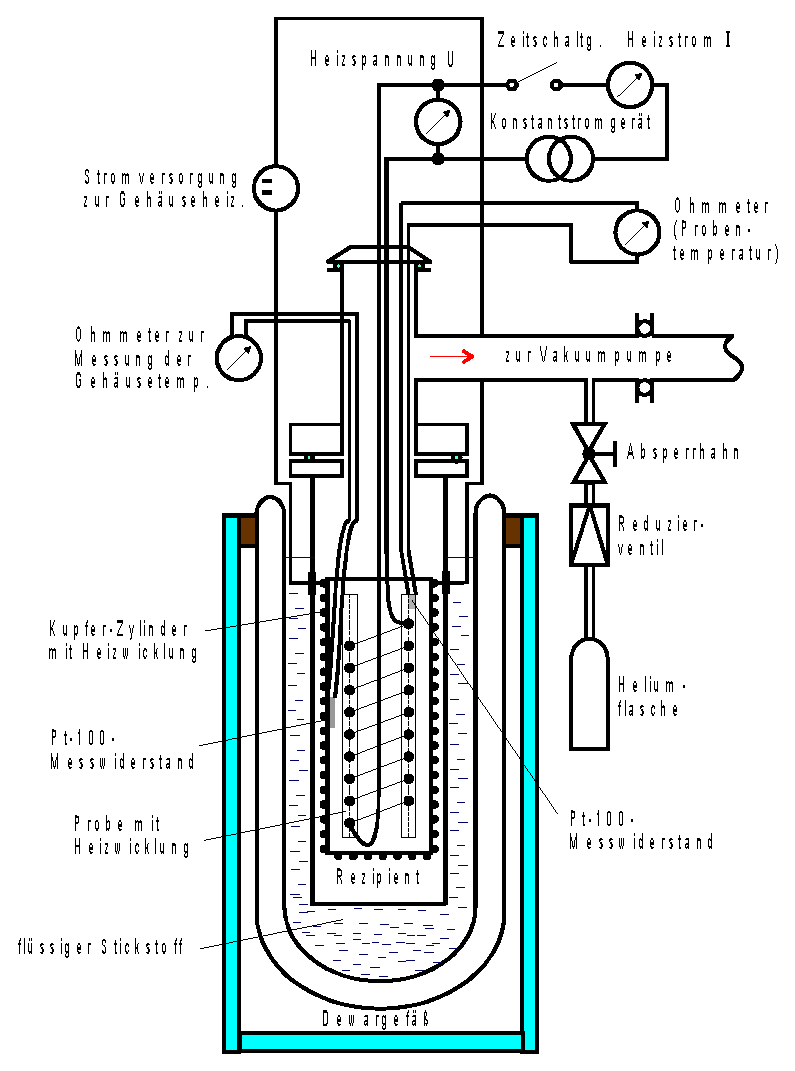
\includegraphics[width=0.5\textwidth]{Aufbau.pdf}
        \caption{Simplified representation of the used apparatus \cite{ap47}.}
        \label{fig:Aufbau}
\end{figure}
The heart of this setup is the with liquid nitrogen filled Dewar vessel. The copper cylinder is placed inside of it. In order to be in control of the samples's temperature, it is surrounded by a heating coil.
The temperature is measured by two PT-100 measuring resistors whose electrical resistant changes monotonically with temperature.
The mathematical equation that puts resistance and temperature in relation is given by 
\begin{equation*}
    T=0.00134 R^2+2.296*R-243.02+ 273.15\; . 
\end{equation*}
The recipient is connected to a vacuum pump and a helium supply during cooling. Both sample and cylinder are supplied with a heating voltage.


\subsection{Measurement method}
The first step is to evacuate the recipient to prevent the liquefaction of air in the cylinder due to low temperatures.
Secondly, helium is filled in because it does not liquify at temperatures at about $T=80\, \unit{\kelvin}$. Further helium has a good thermal conductivity.
As mentioned the temperature to start with is $T=80\, \unit{\kelvin}$, when T is reached the recipient is evacuated again to reduce pressure even further and decrease loss due to conductivity, evaporation and radiation.
Then energy in form of heat (by increasing the heating voltage) is put into the system which leads to a rise in temperature.  
The $\Delta T$ is supposed to be between $7-11\,\unit{\kelvin} $ to prevent exalted heat loss due to a high temperature gradient.
Afterwards, the copper cylinder is heated to the same temperature as the recipient.
To determine the molar heat capacity of copper between  $T=80\, \unit{\kelvin}$ and $T=300\, \unit{\kelvin}$, temperature needs to be gradually increased while measuring time, voltage and heating current are recorded.
Important: Presssure is kept at atmospheric pressure during the duration of the measurement.
%\section{Durchführung}
\label{sec:Durchführung}


\section{Analysis of the Experimental data}
\label{sec:Auswertung}

\subsection{Fehlerrechnung}
\label{sec:Fehlerrechnung}
Für die Fehlerrechnung werden folgende Formeln aus der Vorlesung verwendet.
für den Mittelwert gilt
\begin{equation}
    \overline{x}=\frac{1}{N}\sum_{i=1}^N x_i ß\; \;\text{mit der Anzahl N und den Messwerten x} 
    \label{eqn:Mittelwert}
\end{equation}
Der Fehler für den Mittelwert lässt sich gemäß
\begin{equation}
    \increment \overline{x}=\frac{1}{\sqrt{N}}\sqrt{\frac{1}{N-1}\sum_{i=1}^N(x_i-\overline{x})^2}
    \label{eqn:FehlerMittelwert}
\end{equation}
berechnen.
Wenn im weiteren Verlauf der Berechnung mit der fehlerhaften Größe gerechnet wird, kann der Fehler der folgenden Größe
mittels Gaußscher Fehlerfortpflanzung berechnet werden. Die Formel hierfür ist
\begin{equation}
    \increment f= \sqrt{\sum_{i=1}^N\left(\frac{\partial f}{\partial x_i}\right)^2\cdot(\increment x_i)^2}.
    \label{eqn:GaussMittelwert}
\end{equation}

\section{Discussion}
\label{sec:Diskussion}


\newpage
\printbibliography
\nocite{ap47}
\nocite{matplotlib}
\nocite{numpy}
\nocite{scipy}
\nocite{uncertainties}
\nocite{reback2020pandas}

\newpage
%\includepdf[scale=0.7,pages=1,pagecommand=\section*{Anhang}\thispagestyle{empty}]{messdaten.pdf}
%\addcontentsline{toc}{section}{\protect\numberline{}Anhang}
%\includepdf[scale = 0.7, pages=-]{messdaten.pdf}

\end{document}
